\section{Coq}

En este capitulo introduciremos las características más relevantes del asistente de pruebas interactivo Coq. El objetivo de este capitulo es introducir todos los conceptos que utilizaremos más adelante, pero esto significa que no es una introducción completa.

El desarrollo de Coq comenzó en 1984 con el apoyo de INRIA como el trabajo de Gérard Huet y Thierry Coquand. En ese momento Coquand estaba implementado un lenguaje llamado \textit{Calculus of Constructions} cuando el 1991 una nueva implementación basada en un Calculus of Inductive Constructions extendido comenzó a ser desarrollado tomando el nombre de Coq.

Ahora mismo Coq es desarrollado por más de 40 desarrolladores activos y es reconocido como unos de los asistentes de prueba principales.

Como un asistente de pruebas la orientación de Coq es la de permitir la escritura totalmente formal de teoremas y pruebas, y asegurarnos de su correción. Se parte de lo que se denomina \textit{kernel}, el nucleo de Coq, que es el que verifica que la prueba corresponde al teorema, es decir, que sea correcta. De esta forma, el humano no está encargado de verificar la prueba, solo de escribirla.
% TODO: diferencia con otros asistentes

\subsection{Los lenguajes Coq}

Coq no es técnicamente un lenguaje de programación, si no un asistente de pruebas. Pero podemos encontrar múltiples lenguajes dentro de Coq que nos permiten expresarnos. 
\begin{itemize}
    % TODO: cita Gallina? http://adam.chlipala.net/cpdt/html/Universes.html
    \item \textit{Gallina}: este es el lenguaje de especificación de Coq. Permite desarrollar teorías matemáticas y probar especificaciones de programas. Utilizaremos extensivamente un lenguaje muy similar a este para definir nuestros programas en Mtac2.
    % TODO: cita Ltac?
    \item \textit{Ltac}: este el lenguaje en que se definen las \textit{tácticas} de Coq. Dado que Coq está centrado en las tácticas, Ltac es una de las partes centrales del aparato.
    \item \textit{Vernacular}.
\end{itemize}

Aunque Coq no es un lenguaje de programación propiamente dicho, este puede ser utilizado como un lenguaje de programación funcional. Estos programas serán especificados en Gallina. Dada la naturaleza de Coq como provador de teoremas, estos programas son funciones puras, es decir, no producen efectos secundarios y siempre terminan.

\subsection{La teoría de Coq}

\textit{Calculus of Inductive Constructions} es la base de Coq. Este es un cálculo lambda tipado de alto orden y puede ser interpretado como una extensión de la correspendencia Curry-Howard.

Llamaremos \textit{Terms} (o términos) a los elementos básicos de esta teoría. Terms incluye \textit{Type}, \textit{Prop}, variables, tuplas, funciones, entre otros. Estás son algúnas de las herramientas que utilizaremos para escribir nuestros programas.

% TODO: Ampliar sobre las capacidades de Coq.

\subsection{Tipos de datos y Funciones}

Ahora aprenderemos a codificar nuestros programas funcionales en Coq. Lo primero que debemos entender es que operamos sobre \textit{términos} y algo es un término si tiene tipo. Coq provee muchos tipos predefinidos, por ejemplo \lstinline{unit}, \lstinline{bool}, \lstinline{nat}, \lstinline{list}, entre otros. A continuación estudiaremos cómo definir tipos y funciones.

Veamos cómo se define el tipo \lstinline{bool}:
\begin{lstlisting}
Inductive bool : Set :=
  | true : bool
  | false : bool.
\end{lstlisting}
Como podemos observar, es un tipo inductivo, especificado por la keyword \lstinline{Inductive}, con dos constructores \lstinline{true} y \lstinline{false}. De por sí, el tipo \lstinline{bool} no posee un significado hasta que nosotros lo proveamos de uno. Podemos ahora intentar definir algunos operadores booleanos.
\begin{lstlisting}
Definition andb (b1 b2:bool) : bool := if b1 then b2 else false.
Definition orb (b1 b2:bool) : bool := if b1 then true else b2.
Definition implb (b1 b2:bool) : bool := if b1 then b2 else true.
Definition negb (b:bool) := if b then false else true.
\end{lstlisting}
Las definiciones de funciones no recursivas comienzan con el keyword \lstinline{Definition}. La primera se llama \lstinline{andb} y toma dos booleanos como argumentos y retorna un booleano. Se utiliza la notación \lstinline{if b then x else y} para matchear sobre los booleanos de manera más fácil. Finalmente podemos definir una función más interesante.
\begin{lstlisting}
Definition Is_true (b:bool) :=
  match b with
    | true => True
    | false => False
  end.
\end{lstlisting}

Ahora, veamos un tipo con un ingrediente un poco más complicado, \lstinline{nat}.
\begin{lstlisting}
Inductive nat : Set :=
  | O : nat
  | S : nat -> nat.
\end{lstlisting}
Notemos que el constructor \lstinline{S} es una función que recibe un término de tipo {nat}, es decir, \lstinline{nat} es un tipo recursivo. Por ejemplo el término \lstinline{S (S O)} es de tipo \lstinline{nat} y representa al número 2.

Para continuar con este desarrollo, veamos el tipo de \lstinline{list} que es polimórfico.
\begin{lstlisting}
Inductive list (A : Type) : Type :=
  | nil : list A
  | cons : A -> list A -> list .
\end{lstlisting}
Este tipo es un tipo polimórfico dado que requiere de un \lstinline{A : Type}. Por ejemplo, una posible lista es \lstinline{cons (S O) nil : list nat} que representa a la lista con un único elemento 1 de tipo \lstinline{nat}.

Definiremos una función que añade un elemento a una lista.
\begin{lstlisting}
Definition add_list {A} (x : A) (l : list A) : list A :=
  cons x l.
\end{lstlisting}
Dado que el tipo \lstinline{A} puede ser inferido facilmente por Coq, utilizamos llaves a su alrededor para expresar que sea un argumento implícito. En el cuerpo de la función solo utilizamos \lstinline{cons}, uno de los constructores de \lstinline{list}, para añadir un elemento delante de \lstinline{l}.

Ahora nos interesa definir la función \lstinline{length} que retorna el largo de una lista.
\begin{lstlisting}
Fixpoint len {A} (l : list A) : nat :=
match l with
| [] => O
| x :: xs => S (len xs)
end.
\end{lstlisting}
Coq está diseñado de forma que necesitamos utilizar el keyword \lstinline{Fixpoint} para poder definir funciones recursiva. Aquí Coq está encontrando el argumento decreciente de la función \lstinline{len} y por eso acepta nuestra definición. El cuerpo de \lstinline{len} inspecciona a \lstinline{l} y lo \textit{matchea} con el caso correspondiente. Utilizamos \lstinline{S} y \lstinline{O}, los constructores de \lstinline{nat} para expresar el valor de retorno.

\subsection{Tipos dependientes}

Una de las herramientas más importantes que hay en Coq son los tipos dependientes. Estos nos permiten hablar de elementos que dependen de otros anteriores. Por ejemplo, puede ser de nuestro interés hablar de números positivos, en otras palabras, \lstinline{x : nat} tal que \lstinline{x <> O}. En este caso, \lstinline{x <> O} es una prueba que depende de \lstinline{x} y solo existirá cuando \lstinline{x} sea mayor a 0.

Para hablar de un ejemplo práctico de tipos dependientes, hemos elegido la función \lstinline{head} que retorna la cabeza de una lista. Comencemos con la versión más simple, donde utilizamos un valor default \lstinline{d} para el caso en que la lista es vacía.
\begin{lstlisting}
Definition head_d {A} (l : list A) (d : A) : A :=
  match l with
  | [] => d
  | x :: xs => x
  end.
\end{lstlisting}
El problema de esta solución es que a excepción de que \lstinline{d} sea un valor único, no hay manera de saber si la función retornó realmente la cabeza de la lista.

La segunda opción es utilizar el tipo \lstinline{option}.
\begin{lstlisting}
Inductive option A : Type :=
| None : option A
| Some : A -> option A.
\end{lstlisting}
Con este tipo auxiliar podemos reescribir \lstinline{hd}.
\begin{lstlisting}
Definition head_o {A} (l : list A) : option A :=
  match l with
  | [] => None
  | x :: xs => Some x
  end.
\end{lstlisting}
Esta solución es mejor que la anterior pero sigue sufriendo de una deficiencia. Dado que \lstinline{head_o} retorna un \lstinline{option} no sabemos si el resultado de esta función será realmente un elemento o si será el constructor vacío, por lo que todas las funciones que utilicen a \lstinline{head_o} deben también utilizar \lstinline{option}.
% TODO: citar? failure is not an option

Esto nos lleva a nuestra última solución. Esta requiere que nos aseguremos que la lista \lstinline{l} no es vacia, es decir, \lstinline{l <> []}. Pero para entenderla debemos ver dos cosas más: $\Sigma$\textit{-types} y \lstinline{Program}.
% TODO: sigma types.
Intuitivamente, los $\Sigma$\textit{-types} son tuplas donde el argumento de la derecha es dependiente del de la izquierda. A continuación, la definición.
\begin{lstlisting}
Inductive sig (A : Type) (P : A -> Prop) : Type :=
  exist : \forall x : A, P x -> {x : A | P x}
\end{lstlisting}
Se utiliza la notación \lstinline|{x : A \| P x}| para expresar \lstinline{sig A (fun x => P)}.
% TODO: está bien la notación?

\lstinline{Program} es una libreria que permite progamar en Coq como si fuera un lenguaje de programación funcional mientras que se utiliza una especificación tan rica como se desee y probando que el codigo cumple la especificación utilizando todo el mecanizmo de Coq. En nuestro caso utilizaremos \lstinline{Program} para codificar \lstinline{head} de una manera casi transparente.
\begin{lstlisting}
Program Definition head {A}
(l : list A | [] <> l ) : A :=
  match l with
  | [] => !
  | x :: xs => x
  end.
\end{lstlisting}
Como podemos observar, la única diferencia es que la signatura de \lstinline{head} especificamos que \lstinline{l} es una lista junto con una prueba que muestra que no es vacía.

\subsection{Tácticas}

En la próxima sección hablaremos de pruebas, metas (\textit{goals}) y tácticas. Para esto introduciremos un ejemplo que nos facilite entender estos conceptos.

\begin{exmp}\label{exmp:sub_0_r}
\begin{lstlisting}
Lemma sub_0_r : forall n, n - 0 = n.
Proof. intro n. case n; [ | intro n']; reflexivity. Qed. 
\end{lstlisting}
\end{exmp}

% TODO: cita Ltac https://coq.inria.fr/refman/zebibliography.html#del00
% TODO: Utilizar tácticas de Coq. Mencionar que hay múltiples librerías de tacticas.

El teorema a probar restar 0 a cualquier número $n$ es $n$. Ya que la resta está definida por pattern matching en el primer argumento, esta igualdad no es automáticamente cierta computando. Por eso, debemos hacer análisis por casos.

El código comienza con el comando \lstinline{Lemma}, donde efectivamente definimos lo que queremos probar.
Luego utilizamos el comando \lstinline{Proof} para indicar el inicio de la prueba, la cual será resuelta a través de la concatenación de tácticas de Ltac. Estas tácticas trasnforman el \textit{proof-state} incrementalmente construyendo un \textit{proof-term}, la prueba.

Después de \lstinline{Proof}, Coq genera una \lstinline{goal}, una meta. Internamente, una meta en Coq es representada con una \textit{meta-variable}. Esta meta-variable tiene un tipo, en concreto el lema que queremos probar. En este caso nuestra meta $?g$ tiene tipo \lstinline{\forall n, n - 0 = n}.

Para introducir la variable $n$, utilizamos \lstinline{intro}. Esta instancia a $?g$ como \lstinline{fun n:nat => $?g_1$} donde el tipo de $?g_1$ es \lstinline{n - 0 = n}.

% TODO: Contextual Modal Type Theory, Nanevsky 2008.
Ya introducida la variable, el próximo paso es hacer análisis por casos en ella. Con \lstinline{case} podemos analizar a $n$ según los constructores de su tipo. Para el primer caso: \lstinline{0 - 0 = 0} es trivial. El segundo caso es \lstinline{\forall n':nat, S n' - 0 = S n'}, para el cual, primero introduciremos $n'$ y luego, por la naturaleza inductiva de la resta, será igualmente trivial para Coq. La táctica \lstinline{case} retorna estas dos sub-metas, las cuales componemos, con el operador de composición (el punto y coma), con las tácticas listadas en \lstinline{[ | intro n']}. La primer sub-meta es resuelta por la táctica a la izquierda del \lstinline{|}, que es implicitamente la táctica identidad (\lstinline{idtac}), mientras que la segunda sub-meta es resuelta por la táctica a la derecha de \lstinline{|}, \lstinline{intro n'}. La salida de esta composición son de nuevo dos tácticas las que de nuevo compondremos con \lstinline{reflexivity}. Esto signfica que aplicaremos \lstinline{reflexivity} a ambas tácticas resultantes, resolviendolas trivialmente por computación.

\subsection{Interfaz interactiva}

Cuando se dice que Coq es un asistente \textit{interactivo} nos referimos a que Coq nos puede ayudar a desarrollar la prueba en cierta medida.
% TODO: UI de Coq, dar ejemplos.
Por ejemplo, supongamos que queremos probar el siguiente teorema.
\begin{exmp}
\begin{lstlisting}
Definition le_S (n : nat) : n <= S n.
\end{lstlisting}
\end{exmp}
Al entrar a alguno de los editores de textos compatibles con Coq (Emacs, Visual Studio Code o CoqIDE) cargamos el teorema y Coq entrará al modo interactivo, en el cual nos mostrará el estado actual de la prueba. En este caso comenzamos con la hipótesis \lstinline{n : \nat} ya en nuestro contexto y una única meta $?g$ de tipo \lstinline{n <= S n}. Ahora aplicamos inducción en \lstinline{n} obteniendo dos sub-metas: $?g_1$ con tipo \lstinline{0 <= S 0} y $?g_2$ con tipo \lstinline{S n <= S (S n)}. Para la primera meta $?g_1$ utilizamos \lstinline{apply} para aplicar el teorema \lstinline{le_0_n} instanciado con \lstinline{S n}, esto soluciona automaticamente la sub-meta. La segunda sub-meta se resuelve de una manera similar, solo que tenemos una hipótesis inductiva \lstinline{IHn}.

En la figura \ref{fig:ui} podemos observar como se nos presenta esta información.

\begin{figure}[h]
  \centering
  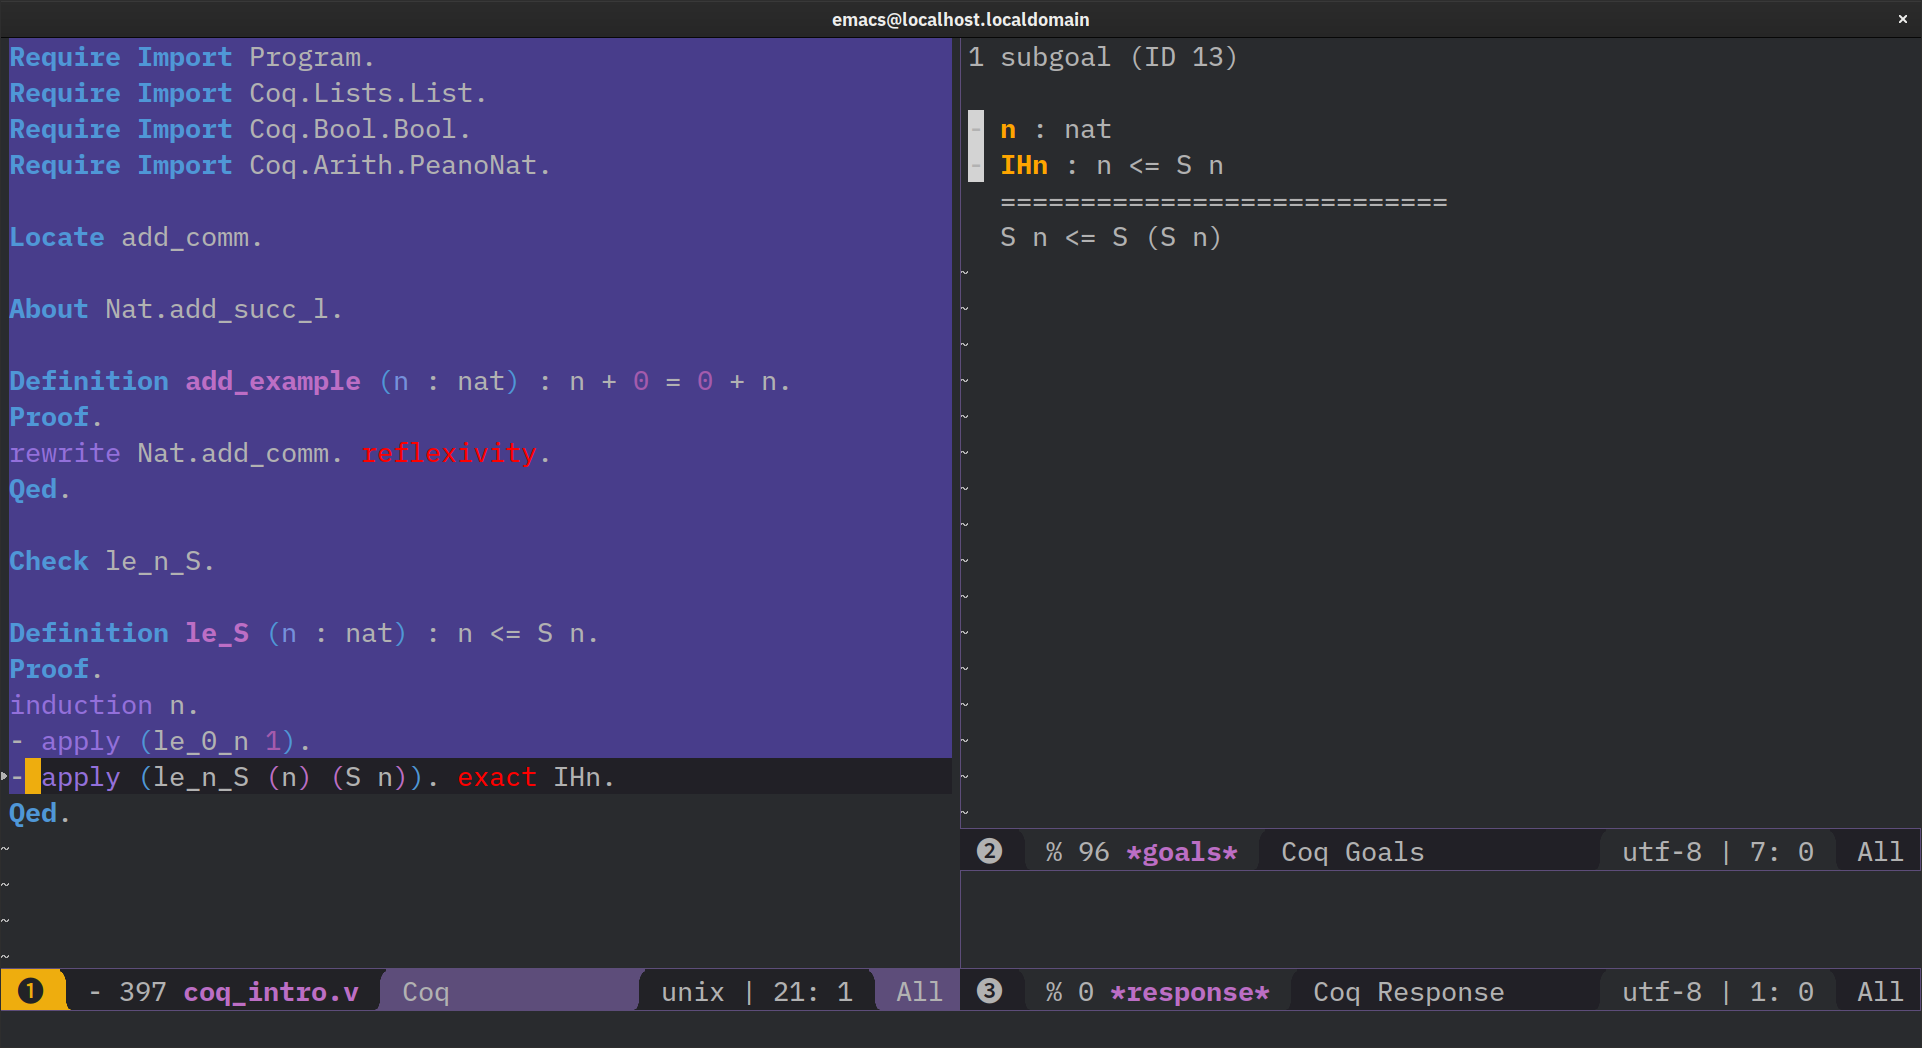
\includegraphics[width=1\textwidth]{gfx/coq_emacs_example.png}
  \caption{Ejemplo de interfaz de Coq}
  \label{fig:ui}
\end{figure}

Coq cuenta con muchos comandos que se usan constantemente.
\begin{itemize}
  \item \lstinline{Check} imprime el tipo de un término. Cuando es llamado en modo prueba, el término es chequeado en el contexto local de la sub-meta.
  \item El comando \lstinline{About} muestra información general.
  \item \lstinline{Print}:
  \item \lstinline{Locate}:
  \item \lstinline{Eval}:
\end{itemize}